\subsection{PC}

\begin{figure}[H]
\centering
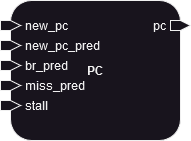
\includegraphics[width=0.5\textwidth]{../diagrams/fetch/pc.png}
\caption{Diagram of the PC}
\label{fig:PC}
\end{figure}

The PC is responsible for computing the next PC. It uses the different input signals to know which PC to compute.
for example, if it is a branch, the branch predictor will tell him what to do, and if the branch predictor is wrong
it will be updated accordingly. If it is a more classic instruction such as an ADD, it will simply increment the PC by 4
etc. \\

Signals:
\begin{enumerate}
    \item Input: $new\_pc$, This signal represent the next PC given by the branch unit in the EX stage.
    \item Input: $new\_pc\_pred$, This signal represent the next PC given by the branch predictor.
    \item Input: $br\_pred$, This signal is representing the state of the prediction made by the branch predictor in the EX stage.
    \item Input: $miss\_pred$, This signal is representing if there is a miss prediction or not.
    \item Input: $stall$, This signal is representing if the pipeline is stalled or not due to a data dependency in the ID stage.
    \item Output: $pc$, This signal is representing the current PC.
\end{enumerate}